\documentclass[11pt]{article}
\usepackage{notes-common}

% Diagram convention used throughout: field arrows live in one band, label
% leaders in another. If a leader crosses an arrow the student cannot tell
% which thing the blank belongs to.

\begin{document}

\noteshead{More Gauss's Law --- the Three Symmetries}{PHYS 230/235 \quad$\cdot$\quad Wed Sep 23 \quad$\cdot$\quad Knight 24.4--24.6}
\nameline

\goal{State Gauss's law and understand what it says, then use it to \emph{compute}
$\vec{E}$ --- not just check it --- for the distributions where symmetry makes that
possible: a point charge and a shell, an infinite line, an infinite sheet, and a
uniformly charged sphere.}

%============================================================
\nsec{What Gauss's law says}

\emph{Flux} $\Phi$ counts electric field lines crossing a surface: a line leaving counts
$+1$, a line entering counts $-1$, so a line that just passes through contributes
\bl[1.2cm]\ net. For a \textbf{closed} surface,
\[
\Phi = \oint \vec{E}\cdot d\vec{A} \ \Big(= \oint E\cos\theta\, dA,\ \ \theta\text{ between
}\vec E\text{ and the outward normal}\Big),\qquad d\vec{A}\text{ always points \bl[1.8cm].}
\]

Gauss's law says that count is fixed by exactly one thing:
\[
\Phi = {}\bl[3.2cm]
\]
not the surface's size, not its shape, not how far it is from the charge.

\checkpoint{A point charge sits at the center of a Gaussian sphere. If you double the
sphere's radius, does $\Phi$ change? Does $E$ at the surface change? (Different questions!)}

%============================================================
\nsec{Using it: match the surface to the symmetry}

Gauss's law holds for \emph{any} closed surface, but it only lets you \emph{solve} for $E$
when you can pull $E$ outside the integral. Choose a Gaussian surface that shares the
charge distribution's own symmetry --- \textbf{spherical}, \textbf{cylindrical}, or
\textbf{planar} --- centered or aligned on the distribution, and two things become true
everywhere on it:
\begin{enumerate}[leftmargin=*, itemsep=1.5mm, topsep=1mm]
  \item $E$ has the same \bl[3cm]\ everywhere on it, and
  \item $\vec{E}$ is everywhere either \bl[2.4cm]\ or \bl[2.4cm]\ to the surface.
\end{enumerate}
Then $\Phi = E\oint dA = EA$, and Gauss's law becomes plain algebra: $EA=q_{\text{enc}}/\varepsilon_0$.

{\small\color{blankink}\textit{What ``symmetric'' means:} if you closed your eyes while
the charge distribution changed in a symmetric way, then opened them again, you
couldn't tell anything had changed.}

\checkpoint{Why does a cube fail as a Gaussian surface for a single point charge?}

\newpage
%============================================================
\nsec{Warm-up: a point charge, then a shell}

\begin{center}
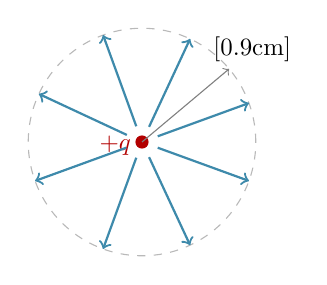
\begin{tikzpicture}[x=0.85cm,y=0.85cm]
  \filldraw[red!70!black] (0,0) circle (0.09);
  \node[red!70!black, scale=0.9] at (-0.4,-0.05) {$+q$};
  \draw[gray!55, dashed] (0,0) circle (1.7);
  \foreach \a in {20,65,110,155,200,250,295,340}{
    \draw[cyan!65!black, ->, line width=0.8pt] (\a:0.25) -- (\a:1.7);}
  \draw[gray, ->] (0,0) -- (40:1.7);
  \node[scale=0.9] at (40:2.15) {\dlabel[0.9cm]};
\end{tikzpicture}
\end{center}
\figtask{Label the Gaussian radius $r$.}

By symmetry $\vec E$ is radial and constant in magnitude on the sphere, so
$EA=q_{\text{enc}}/\varepsilon_0$ with $A=4\pi r^2$ and $q_{\text{enc}}=q$ gives
$E={}$\bl[2.6cm] --- Coulomb's law, recovered from Gauss's law.

Now make it a thin \textbf{shell} of charge $Q$, radius $R$, instead of a point.
\textbf{Outside} ($r>R$): the Gaussian sphere encloses \bl[1.5cm], so
$E={}$\bl[2.6cm] (identical to a point charge --- the shell might as well not have a
size). \textbf{Inside} ($r<R$): the Gaussian sphere encloses \bl[1.5cm], so
$E={}$\bl[1.5cm].

\checkpoint{The sphere you'll work below is \emph{solid}, not a shell --- charge fills
the whole volume. Will its field inside behave the same way as the shell's?}

%============================================================
\nsec{Infinite line of charge}

Linear charge density $\lambda$. $\vec{E}$ points radially out from the wire and cannot
depend on position along it, so the Gaussian surface is a \emph{coaxial cylinder} of
radius $r$ and length $L$.

\begin{center}
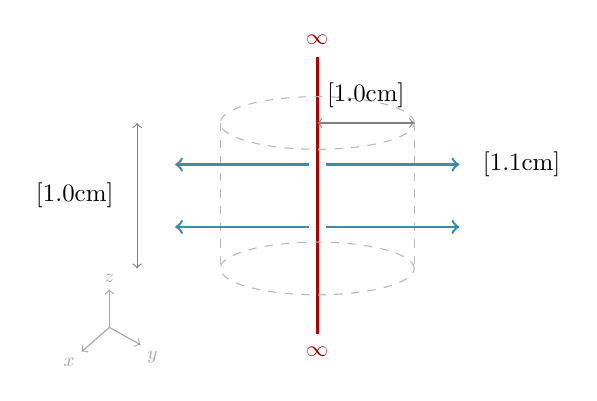
\begin{tikzpicture}[x=0.88cm,y=0.88cm]
  % --- the wire
  \draw[red!70!black, line width=1.1pt] (0,-2.0) -- (0,2.0);
  \node[red!70!black, scale=0.8] at (0,2.25) {$\infty$};
  \node[red!70!black, scale=0.8] at (0,-2.25) {$\infty$};
  % --- Gaussian cylinder
  \draw[gray!55, dashed] (-1.4,1.05) -- (-1.4,-1.05);
  \draw[gray!55, dashed] (1.4,1.05) -- (1.4,-1.05);
  \draw[gray!55, dashed] (0,1.05) ellipse (1.4 and 0.38);
  \draw[gray!55, dashed] (0,-1.05) ellipse (1.4 and 0.38);
  % --- field arrows: one band only, at y = +-0.45
  \foreach \y in {-0.45,0.45}{
    \draw[cyan!65!black, ->, line width=0.9pt] (0.12,\y) -- (2.05,\y);
    \draw[cyan!65!black, ->, line width=0.9pt] (-0.12,\y) -- (-2.05,\y);
  }
  \node[scale=0.9] at (2.95,0.45) {\dlabel[1.1cm]};      % what are these arrows?
  % --- radius leader, up at cap level, clear of the arrows
  \draw[gray, <->] (0,1.05) -- (1.4,1.05);
  \node[scale=0.9] at (0.7,1.45) {\dlabel[1.0cm]};
  % --- length leader, off to the left
  \draw[gray, <->] (-2.6,-1.05) -- (-2.6,1.05);
  \node[scale=0.9] at (-3.5,0) {\dlabel[1.0cm]};
  % --- orientation triad, tucked in the clear corner below the length leader:
  % the wire runs along z, so this shows the whole picture is a 3D scene seen
  % from an angle, not a flat 2D drawing.
  \draw[gray!70, ->] (-3.0,-1.9) -- (-3.0,-1.35) node[above, scale=0.7] {$z$};
  \draw[gray!70, ->] (-3.0,-1.9) -- (-3.4,-2.25) node[below left, scale=0.7] {$x$};
  \draw[gray!70, ->] (-3.0,-1.9) -- (-2.55,-2.15) node[below right, scale=0.7] {$y$};
\end{tikzpicture}
\end{center}
\figtask{Label the cylinder's radius, its length, and the field arrows. (The wire runs
along $z$ --- this is a 3D picture, seen at an angle.)}

\derivbox{2.9cm}{Which part of the cylinder carries flux (and which carries none)? Area $A$, then $q_{\text{enc}}$, then solve for $E$. Show $L$ cancelling.}

\result{$E$ for an infinite line}

\newpage
%============================================================
\nsec{Infinite sheet of charge}

Surface charge density $\eta$. This is a \emph{plane}, not a line: it extends forever in
\emph{two} directions, $x$ and $y$, and $\vec{E}$ points straight away from it along $\pm z$
on both sides.

\begin{center}
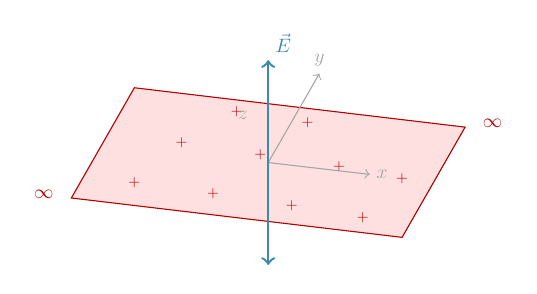
\begin{tikzpicture}[x=1cm,y=1cm]
  % --- the sheet in perspective: a tilted parallelogram, so it visibly extends
  % in two directions instead of reading as a 1D line. A,B,C,D chosen so
  % AB = DC and AD = BC (a genuine parallelogram, not just four points).
  \fill[red!12] (-2.4,-0.4) -- (1.8,-0.9) -- (2.6,0.5) -- (-1.6,1.0) -- cycle;
  \draw[red!70!black] (-2.4,-0.4) -- (1.8,-0.9) -- (2.6,0.5) -- (-1.6,1.0) -- cycle;
  \foreach \p in {(-1.6,-0.2),(-0.6,-0.35),(0.4,-0.5),(1.3,-0.65),
                  (-1.0,0.3),(0.0,0.15),(1.0,0.0),(1.8,-0.15),
                  (-0.3,0.7),(0.6,0.55)}{
    \node[red!70!black, scale=0.55] at \p {$+$};}
  \node[red!70!black, scale=0.7] at (-2.75,-0.35) {$\infty$};
  \node[red!70!black, scale=0.7] at (2.95,0.55) {$\infty$};
  % --- in-plane axes x,y, along the sheet's own edge directions
  \coordinate (O) at (0.1,0.05);
  \draw[gray!70, ->] (O) -- ++(1.29,-0.15) node[right, scale=0.7] {$x$};
  \draw[gray!70, ->] (O) -- ++(0.65,1.13) node[above, scale=0.7] {$y$};
  % --- the field, straight out of the plane both ways --- this arrow pair
  % doubles as the z axis, so no separate z-arrow is drawn on top of it.
  \draw[cyan!65!black, ->, line width=0.9pt] (O) -- ++(0,1.3) node[above right, scale=0.7, cyan!65!black] {$\vec E$};
  \node[gray!70, scale=0.7] at (-0.22,0.65) {$z$};
  \draw[cyan!65!black, ->, line width=0.9pt] (O) -- ++(0,-1.3);
\end{tikzpicture}
\end{center}
\figtask{An infinite sheet, seen at an angle: it extends forever in $x$ \emph{and} $y$,
and $\vec E$ points straight out along $z$ on either side.}

Now look at it \emph{edge-on} (sighting along $y$, so the sheet appears as a line and the
pillbox is easy to draw), with end caps of area $A_{\text{cap}}$:

\begin{center}
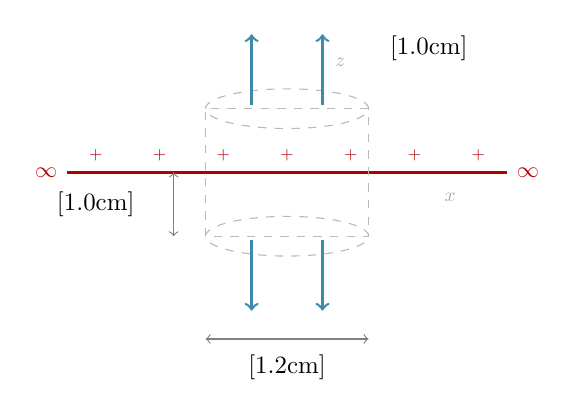
\begin{tikzpicture}[x=0.9cm,y=0.9cm]
  % --- the sheet, edge on. Thin line so the + signs above it stay legible.
  \draw[red!70!black, line width=0.8pt] (-3.1,0) -- (3.1,0);
  \foreach \x in {-2.7,-1.8,-0.9,0,0.9,1.8,2.7}{
    \node[red!70!black, scale=0.62] at (\x,0.24) {$+$};}
  \node[red!70!black, scale=0.8] at (-3.4,0) {$\infty$};
  \node[red!70!black, scale=0.8] at (3.4,0) {$\infty$};
  % --- small tags tying this back to the 3D figure above: the sheet line here
  % is the x direction, seen edge-on; the field arrows are along z.
  \node[gray!70, scale=0.7] at (2.3,-0.35) {$x$};
  \node[gray!70, scale=0.7] at (0.75,1.55) {$z$};
  % --- pillbox
  \draw[gray!55, dashed] (-1.15,-0.9) rectangle (1.15,0.9);
  \draw[gray!55, dashed] (0,0.9) ellipse (1.15 and 0.28);
  \draw[gray!55, dashed] (0,-0.9) ellipse (1.15 and 0.28);
  % --- field arrows, inboard
  \foreach \x in {-0.5,0.5}{
    \draw[cyan!65!black, ->, line width=0.9pt] (\x,0.95) -- (\x,1.95);
    \draw[cyan!65!black, ->, line width=0.9pt] (\x,-0.95) -- (\x,-1.95);
  }
  \node[scale=0.9] at (2.0,1.75) {\dlabel[1.0cm]};
  % --- half-height leader on the LEFT and BELOW the sheet: the + signs all sit
  % above the line, so that quadrant is the only one with nothing in it.
  \draw[gray, <->] (-1.6,-0.9) -- (-1.6,0);
  \node[scale=0.9] at (-2.7,-0.45) {\dlabel[1.0cm]};
  % --- cap-area leader, below everything
  \draw[gray, <->] (-1.15,-2.35) -- (1.15,-2.35);
  \node[scale=0.9] at (0,-2.75) {\dlabel[1.2cm]};
\end{tikzpicture}
\end{center}
\figtask{Label the pillbox half-height, the cap area, and the field arrows.}

\derivbox{2.6cm}{Total area carrying flux, $q_{\text{enc}}$ in terms of $\eta$ and $A_{\text{cap}}$, then $E$.}

\result{$E$ for an infinite sheet}

\checkpoint{Two surprises. $A_{\text{cap}}$ cancelled --- why did it \emph{have} to? And the
answer contains no $r$ at all. What does that say about walking away from the sheet?}

\vspace{2mm}
\textbf{Then: two parallel sheets}, one $+\eta$ and one $-\eta$. Superpose the two fields
you just found --- nothing new to derive.

\begin{center}
\begin{tikzpicture}[x=0.9cm,y=0.9cm]
  \draw[red!70!black, line width=0.8pt] (-2.6,0.9) -- (2.6,0.9);
  \foreach \x in {-2.2,-1.4,-0.6,0.2,1.0,1.8}{
    \node[red!70!black, scale=0.62] at (\x,1.14) {$+$};}
  \draw[blue!60!black, line width=0.8pt] (-2.6,-0.9) -- (2.6,-0.9);
  \foreach \x in {-2.2,-1.4,-0.6,0.2,1.0,1.8}{
    \node[blue!60!black, scale=0.62] at (\x,-1.14) {$-$};}
  \node[scale=0.85] at (0,0) {\dlabel[1.6cm]};
  \node[scale=0.85] at (0,1.95) {\dlabel[1.6cm]};
  \node[scale=0.85] at (0,-1.95) {\dlabel[1.6cm]};
\end{tikzpicture}
\end{center}
\figtask{Write $E$ in each of the three regions: above, between, below.}

\newpage
%============================================================
\nsec{Uniformly charged sphere}

Total charge $Q$ spread uniformly through a solid sphere of radius $R$. There are two
regions, and the only difference between them is $q_{\text{enc}}$.

\begin{center}
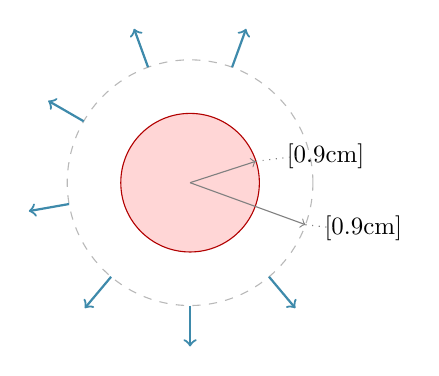
\begin{tikzpicture}[x=0.8cm,y=0.8cm]
  \fill[red!16] (0,0) circle (1.1);
  \draw[red!70!black] (0,0) circle (1.1);
  \draw[gray!55, dashed] (0,0) circle (1.95);
  % field arrows kept to the left/top/bottom so the right side is free for labels
  \foreach \a in {70,110,150,190,230,270,310}{
    \draw[cyan!65!black, ->, line width=0.8pt] (\a:1.95) -- (\a:2.6);}
  % the two radius leaders, both on the clear right-hand side
  \draw[gray, ->] (0,0) -- (18:1.1);
  \node[scale=0.9] at (2.15,0.42) {\dlabel[0.9cm]};
  \draw[gray, dotted] (18:1.1) -- (1.7,0.42);
  \draw[gray, ->] (0,0) -- (-20:1.95);
  \node[scale=0.9] at (2.75,-0.72) {\dlabel[0.9cm]};
  \draw[gray, dotted] (-20:1.95) -- (2.3,-0.72);
\end{tikzpicture}
\end{center}
\figtask{Label the sphere's radius $R$ and the Gaussian radius $r$.}

\textbf{Outside} ($r > R$): the Gaussian sphere encloses \bl[2.4cm]\ of the charge.

\derivbox{2.4cm}{$q_{\text{enc}}$, then $E$. What familiar result does this match?}

\result[1.3cm]{$E$ outside the sphere}

\textbf{Inside} ($r < R$): only the charge within radius $r$ counts. The charge fills the
\bl[2.0cm], so the fraction enclosed is the ratio of \bl[2.4cm].

\derivbox{2.7cm}{$q_{\text{enc}} = {}$?\quad then $E = {}$?}

\result[1.3cm]{$E$ inside the sphere}

\checkpoint{Sketch $E$ against $r$ across both regions. At $r=R$ --- jump, kink, or neither?}

\begin{center}
\begin{tikzpicture}[x=1cm,y=1cm]
  \draw[gray!70, ->] (0,0) -- (7.6,0) node[right, scale=0.8] {$r$};
  \draw[gray!70, ->] (0,0) -- (0,1.9) node[above, scale=0.8] {$E$};
  \draw[gray!35, dashed] (2.5,0) -- (2.5,1.75);
  \node[gray, scale=0.8] at (2.5,-0.32) {$R$};
\end{tikzpicture}
\end{center}

{\small\color{blankink} All three results are in the \emph{Applying Gauss's Law} sim ---
open its \textbf{Info} panel to check yours.}

\end{document}
